\chapter{Implementacja}
Implementacja oparta została o minikomputer Raspberry Pi 4B 2GB. Urządzenie to zostało wybrane losowo - była to platforma, która akurat była dostępna "pod ręką". Na minikomputerze zainstalowany został system operacyjny Linux Ubuntu, w wersji 22.04. System ten był wybrany, jako system wspierany zarówno przez RPi jak i przez środowisko ROS 2. Wersja 22.04 była natomiast najnowszą wersją w czasie rozpoczynania tej części projektu. Bardziej popularny system operacyjny dla tej platformy, czyli Raspbian OS został odrzucony, ponieważ zainstalowanie na nim ROS-a wymaga użycia dockera. Na Ubuntu natomiast wystarczy wykonywać komendy podane wprost w dokumentacji środowiska ROS, co znacznie uprościło podstawową konfigurację środowiska pracy. Wybrana dystrybucja oprogramowania ROS to Humble Hawksbill (rys. \ref{humble_logo}). Podobnie jak w przypadku Ubuntu, wersja ta została wybrana ze względu na fakt, że była to w czasie rozpoczynania prac nad projektem najnowsza. W celu zdalnego łączenia się z minikomputerem użyty został protokół SSH - po stronie RPi otwarty został serwer SSH, a klient (komputer PC) łączył się z nim przy pomocy aplikacji PuTTY. Dodatkowo do sterowania serwami zastosowany został sterownik Polulu Maestro. Urządzenie to zostało wykorzystane ze względu na dostępność i znajomość obsługi.

\begin{figure}[h!]

\includegraphics[width=0.3\textwidth]{img/HumbleHawksbill.png}
\centering
\caption{Logo dystrybucji Humble oprogramowania ROS 2 \cite{ROS_docs}}
\label{humble_logo}
\end{figure}

\section{Środowisko ROS \cite{ROS_docs}}
Robot Operating System (ROS) to zestaw narzędzi programowych służący do tworzenia aplikacji z myślą o robotach. ROS wprowadza sieć niezależnych, działających równolegle, węzłów (ang. node). Węzły te komunikują się za pomoca tematów (ang. topic), które to stanowią niezmienny interfejs między węzłami.\\



Węzły mogą na tematy dane publikować lub je odbierać a implementacja węzła znajdującego się po drugiej stronie nie ma absolutnie znaczenia. Co więcej, nawet nie ma znaczenia czy ten węzeł tam jest. Węzły mogą publikować dane na temty, z których żaden inny węzeł tych danych nie odbiera. Sieć taka jest szczególnie przydatna w przyapdku robotów o pewnym stopniu modularności, bądź w przypadku dowolnych modyfikacji. Zwykle jeden węzeł odpowiada jednemu fizycznemu elementowi robota. Zmiana tego elementu, nawet na element wymagający zupełnie innego oprogramowania, nie jest wtedy problemem. Wystarczy usunąć z sieci odpowiadający mu węzeł i na to miejsce wstawić inny. Jest to bardzo proste, dopóki interfejs (temat na jaki dany węzeł publikuje) pozostaje bez zmian. \cite{ROS_docs}
\subsection{Schemat implementacji}

Rysunek \ref{ros_implementation_schematic} pokazuje schemat komunikacji między poszczególnymi węzłami. Na potrzeby aplikacji zostały stworzone trzy węzły. Jeden odpowiedzialny za obsługę wybranego sterownika do serw-Polulu Maestro, drugi odpowiedzialny za obsługę nogi. Trzeci zaś stanowi główny węzeł sterujący. Ma za zadanie generować algorytm chodu i wysyłać polecenia do nóg, aby układały się na docelowe pozycje.

\begin{figure}[h!]
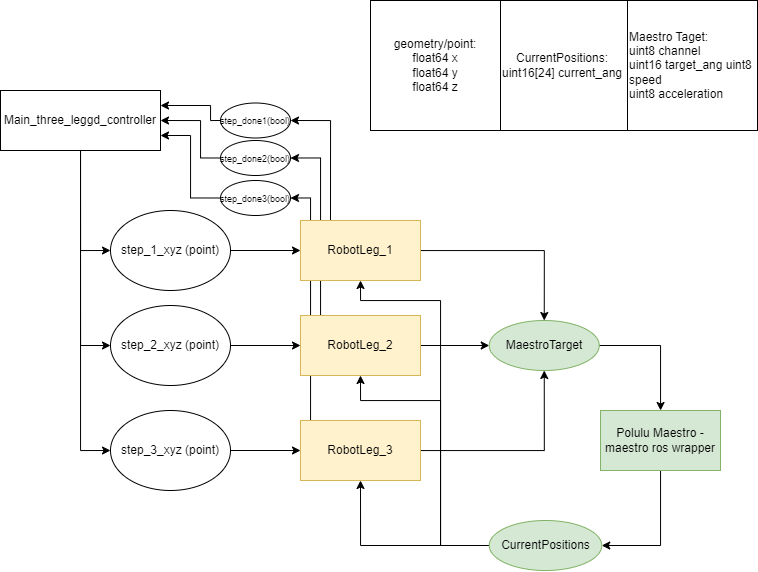
\includegraphics[width=\textwidth]{img/implementation_schematic.png}
\caption{Schemat implementacji w środowisku ROS}
\label{ros_implementation_schematic}
\end{figure}

\section{Polulu Maestro}
Do obsługi serwomechanizmów zastosowany został 24-kanałowy sterownik Polulu Maestro. Do uruchomienia tego robota wystarczyłby oczywiście Polulu Maestro 12 (rys \ref{img:maestro}), lecz wersja 24-kanałowa była zakupiona na potrzebny innego projektu i mogła być tutaj wykorzystana bez dodatkowych wydatków. Natomiast sterowniki do serw firmy Polulu są wymienne, można w każdej chwili przepiąć serwomechanizmy na sterownik o innej ilości kanałów i dokładnie ten sam program będzie w stanie go także obsłużyć. W przyszłości nie będzie problemu z podmianą tego sterownika na mniejszy.\\

\begin{figure}[h!]
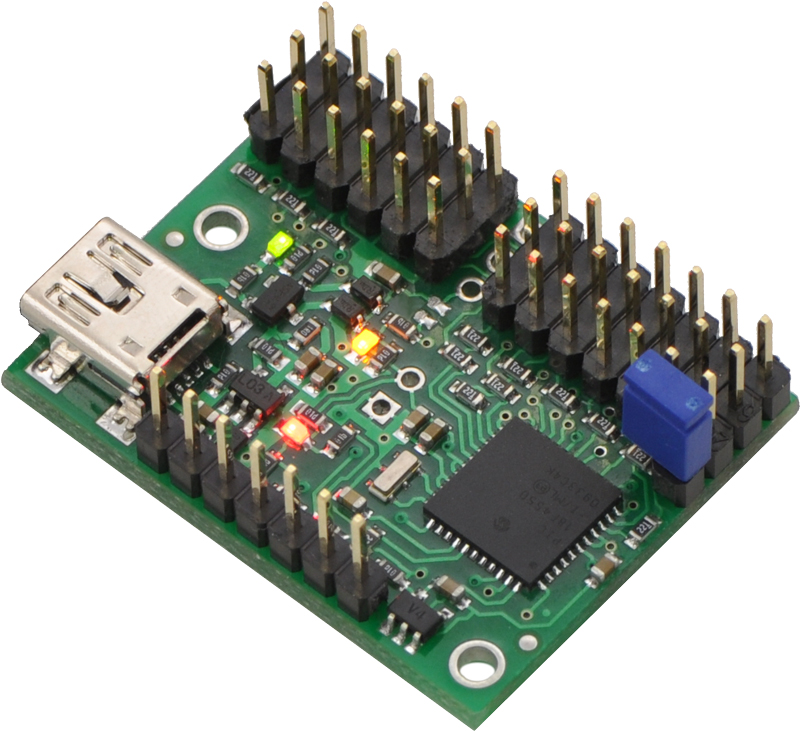
\includegraphics[width=0.4\textwidth]{img/maestro.jpg}
\centering
\caption{Polulu Maestro 12 - kanałowe \cite{maestro_shop}}
\label{img:maestro}
\end{figure}

Komunikacja ze sterownikiem odbywa się za pomocą protokołu UART Serial. Nie było natomiast potrzeby aby tworzyć wiadomości wysyłane tym protokołem od zera, ponieważ istnieje bilbioteka do komunikacji z tym sterownikiem, napisana przez Stevena Jackobsa w języku \texttt{Python} \cite{maestro_pylib}. Jest ona szeroko stosowana w projektach opartych na sterownikach firmy Polulu. W tym projekcie należało jednak otoczyć tą bibliotekę pewnego rodzaju dekoratorem (ang. wrapper) aby połączyć ją z funkcjonalnościami ROSa. Dlatego napisana została klasa \texttt{MaestroRosWrapper} która przez kompozycję zawiera w sobie instancje klasy Maestro z wyżej wymienionej biblioteki Maestro. Stworzona klasa \texttt{MaestroRosWrapper} przede wszystkim implementuje:
\begin{enumerate}[noitemsep]
\item Wysyłanie wiadomości z odczytem obecnej pozcji wszystkich serw
\item Subskrybowanie wiadomości maestro target, która zawiera informacje o:
\begin{itemize}[noitemsep]
\item kanale 
\item pozycji docelowej
\item prędkości
\item przyspieszeniu
\end{itemize}
\end{enumerate}

\begin{figure}[h!]
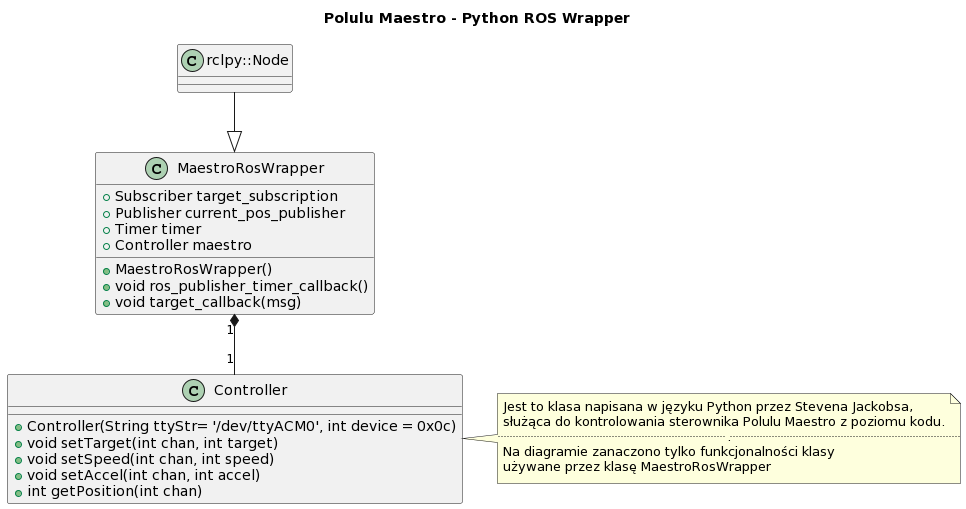
\includegraphics[width=\textwidth]{UML_diagrams/MaestroWrapper.png}
\centering
\caption{diagram UML węzła Polulu Maestro Wrapper}
\label{UML_maestro}
\end{figure}

Na potrzeby tej klasy stworzony został dodatkowy pakiet implementujący dwa niestandardowe (ang. custom) interfejsy:
\begin{itemize}[noitemsep]
\item MaestroTarget
\item CurrentPositions
\end{itemize}
Są to właśnie te dwa wyżej wspomniane interfejsy, za pomocą których węzeł ten komunikuje się ze światem zewnętrznym.\\

Całość kodu służącego do obsługi tego sterownika została napisana w języku \texttt{Python 3}. Język ten został w tym przypadku wybrany, ponieważ Steven Jackobs zaimplementował swoją bibliotekę w tym właśnie języku. Oczywiście przepisanie jej do innego języka (np. \texttt{c++}) nie stanowiłoby dużego problemu, jednakże nie jest to częścią tej pracy. Może to być jednak ciekawe ulepszenie tego projektu, jeżeli węzeł ROS-owy napisany w Pythonie okaże się zbyt pamięciożerny i wolny. Dokładny interfejs stworzonego węzła został przedstawiony na diagramie \ref{UML_maestro}.



\section{Noga Robotyczna}
Poziom wyżej - nad sterownikiem do serw - znajduje się pojedyncza noga robota. Cały program ją obsługujący był pisany na potrzeby tego projektu zupełnie od zera, co dało zupełną dowolność języka i ogólnej struktury implementacji. \\

Jako język został wybrany \texttt{c++}, z powodu ogólnej preferencji autora programu i aby lepiej zoptymalizować całość robota. Pisanie w języku Python jest znacznie prostsze, ale uruchomienie zbyt wielu węzłów napisanych w tym języku może powodować znaczne problemy z wydajnością.\\

Struktura natomiast, była częściowo wzorowana na poprzednim węźle - sterowniku do serw. Także przyjęto zasadę bardziej "generycznej" klasy wewnętrznej i stricte ROS-owego wrappera. W tym przypadku utworzono klasę \texttt{RobotLeg}, przede wszystkim odpowiedzialną za trzymanie informacji o fizycznych parametrach nogi i na ich podstawie przeliczania kinematyk prostej i odwrotnej. Natomiast klasa \texttt{RobotLegWrapper} jest odpowiedzialna za komunikację ze "światem zewnętrznym", czyli innymi węzłami ROS-owymi. Podział ten przedstawiony jest na rys \ref{UML_leg} - diagramie UML tych klas.\\

\begin{figure}[h!]
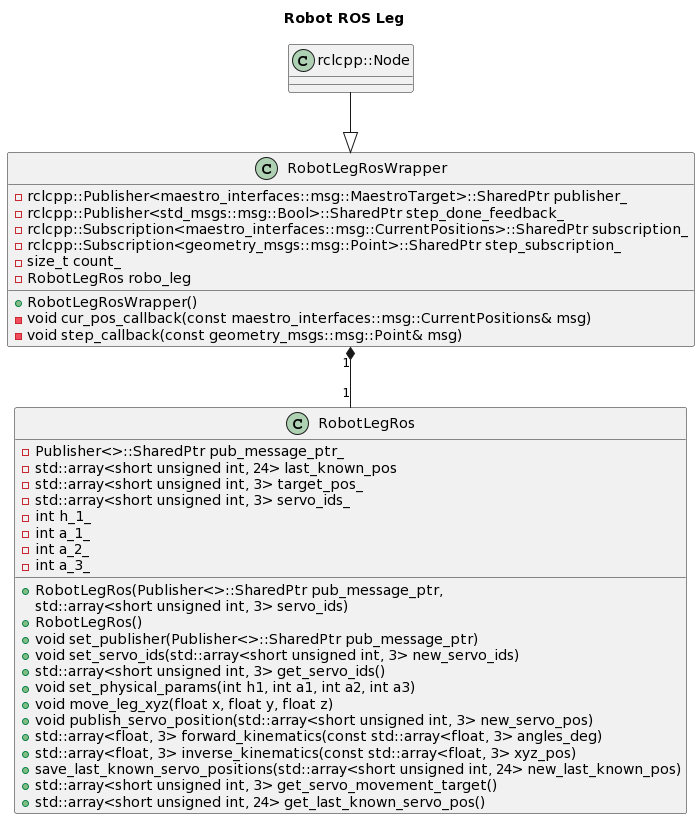
\includegraphics[width=\textwidth]{UML_diagrams/RobotRosLeg.png}
\centering
\caption{diagram UML węzła Robot Leg Ros}
\label{UML_leg}
\end{figure}

Najważniejszymi dwoma interfejsami realizowanymi przez ten węzeł jest przyjmowanie nowej pozycji końcówki robota we współrzędnych kartezjańskich. Jak tylko takowa się pojawi, przeliczana jest kinematyka odwrotna zgodnie ze wzorem \ref{inverse_eq_final} i publikowana jest pozycja w kątach. Dodatkowo, węzeł ten oczekuje sprzężenia zwrotnego od węzła podrzędnego - operującego sterownikiem. Sprzężenie to jest realizowane przez temat zawierający pozycje wszystkich serw. \\

Węzeł ten powinien także zapewnić sprzężenie zwrotne dla węzła nadrzędnego - tego który publikuje nowe pozycje końcówki nogi. Nie jest to jednak pełne sprzężenie zwrotne, takowe nie byłoby możliwe ze względu na fakt, że kinemtyka odwrotna nie jest idealna - zawiera pewien błąd (co zostało dokładnie opisane w rozdziale Model Matematyczny/Noga Robotyczna), natomiast kinematyka prosta nie jest tym błędem obciążona. Prawdziwe sprzężenie zwrotne spowodowałoby, że technicznie rzecz ujmując, noga nigdy by nie osiągnęła punktu docelowego. Dlatego zostało ono uproszczone do wymaganego minimum - jak tylko pojawi się informacja o obecnych pozycjach serw (informacja zwrotna od sterownika) i będą one zgodne z pozycjami docelowymi policzonymi za pomocą kinematyki odwrotnej, to węzeł zmienia wartość w temacie step done typu bool na prawdę. (W czasie wykonywania kroku publikowana jest cyklicznie cały czas wartość fałsz.) Taka informacja zwrotna dla węzła nadrzędnego jest jak najbardziej wystarczająca dla poprawnego ruchu robota.\\

\subsection{Poprawki w interfejsach nogi robotycznej}

Aby uczynić węzeł ten bardziej uniwersalnym i ułatwić jego zastosowanie w innych projektach, można by dodać dwa dodatkowe tematy, na które publikuje ten węzeł - "oszukaną" kinematykę prostą, taką która uwzględnia błąd kinematyki odwrotnej. Dałoby to możliwość zrobienia prawdziwego sprzężenia zwrotnego i liczenia czy krok się faktycznie zakończył wewnątrz węzła nadrzędnego. Byłoby to rozwiązanie bliższe poprawnej "sztuki" implementowania układów sterowania. Dodatkowo warto by było także dodać publikację prawdziwego sprzężenia zwrotnego. Może ono być bardzo przydatne w wielu sytuacjach gdzie potrzebna jest znajomość realnej pozycji końcówki nogi.\\

Innym problemem z interfejsami który wymaga poprawek aby węzeł stał się bardziej uniwersalny są tematy za pomocą których noga komunikuje się ze sterownikiem do serw. Tematy te przenoszą wartości w ćwierć-mikrosekundach, które są jednostką stosowaną przez linię sterowników Polulu Maestro. Powoduje to że konwersja radiany na ćwierć-mikrosekundy jest realizowana już na poziomie nogi robotycznej, a potencjalna wymiana na sterowniki innych producentów może nie być możliwa bez modyfikowania samego kodu nogi. Jest to sprzeczne z ideą ROSa, gdzie wymiana sterownika powinna wiązać się jedynie z wymianą węzła obsługującego ten sterownik. Zamiana tych interfejsów na kąty w stopniach lub radianach i dodanie przeliczania po stronie węzła sterownika poprawiłoby znacznie uniwersalność tej implementacji.\\

Drobnych poprawek wymaga także podział funkcjonalności pomiędzy właściwą klasę \texttt{RobotLeg} a dekorator \texttt{RobotLegROSWrapper}. Jak już wspomniano wcześniej, wrapper ma być odpowiedzialny za komunikację a klasa wewnętrzna za obliczenia. Jednakże na wczesnych etapach implementacji podział ten nie był jeszcze tak jasny i ze względów historycznych, publikacja na temat Maestro Targets jest realizowana przez klasę wewnętrzną. Jest to o tyle problematyczne, że wrapper musi przekazać do klasy wewnątrz wspólny wskaźnik (Shared Pointer), który wskazuje na publishera, na którego temat jest publikowany. Właśnie z tego powodu, i z powodu braku spójności obecnej implementacji, funckjonalność ta powinna być realizowana przez wrapper nie przez klasę wewnętrzną.\\

\section{Klasa kontrolująca trzy nogi i generator trajektorii}
Podobnie jak w przypadku dwóch poprzednich węzłów zastosowano tutaj podział na ROSowego wrappera i klasę implementującą właściwą logikę. Różnicą jest jednak że w przypadku tego węzła klasą "podrzędną" będzie generator trajektorii, który ma za zadanie jedynie generować nowe punkty na które noga ma zostać przestawiona. Jako że istnieje wiele możliwych algorytmów chodu za pomocą których robot ten może się przemieszczać i jednym z celów tego projektu jest stworzenie platformy do eksperymentów z właśnie tymi algorytmami, to należy odpowiednio modularnie zaprojektować interfejs między klasą publikującą a klasą generatora. Modularność taką można bardzo prosto zrealizować korzystając z mechanizmu dziedziczenia. Stworzona została abtrakcyjna klasa Generator3Legs, która implementuje wszystkie podstawowe funkcjonalności generatora jak konstrukctor, ustawianie pozycji początkowych czy obliczanie ruchu konkretnej nogi. Jedna funkcja jest natomiast wirtualna - ta odpowiadająca za faktyczne generowanie kolejnych pozycji kolejnych nóg i zwracanie ich do klasy nadrzędnej. (Tutaj funkcja ta jest nazwana do\_step.) Później napisana została klasa Generator3A która nadpisuje tylko funkcję do\_step. Zależności te zostały przedstawione na diagramie UML na rysunku \ref{UML_controller_generator}\\

\begin{figure}[h!]
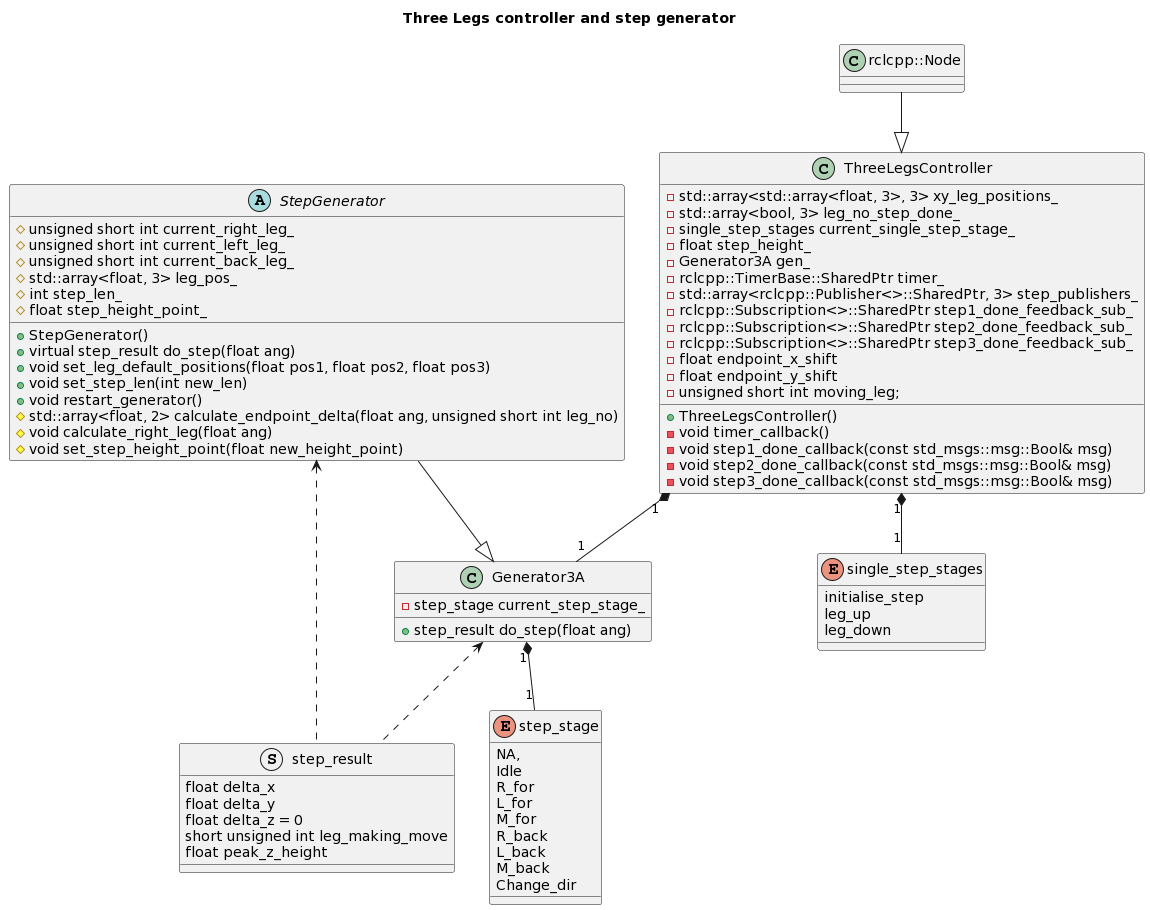
\includegraphics[width=\textwidth]{UML_diagrams/UML_controller_generator.png}
\centering
\caption{diagram UML węzła kontrolera trzech nóg}
\label{UML_controller_generator}
\end{figure}

Dodatkowo implementacja taka umożliwia bardzo ciekawy rozwój projektu. Idąc o krok dalej niż dziedziczenie i stosując mechanizm polimorfizmu, można w czasie rzeczywistym przełączać się między algorytmami. Dodając sterowanie np. za pomocą gamepada, można przyporządkować do kolejnych przycisków zmianę klasy potomnej, która odpowiada za generowanie kroków i zrealizować zmianę algorytmów w czasie pracy robota.\\

Klasa "wrappera" (ThreeLegsController) w przypadku tego węzła ma obecnie funkcjonalność ograniczoną do minimum. Po pierwsze, wywołuje wewnątrz odwołania (ang. callback) od zegara (ang. timer) generowanie kolejnych kroków. Równolegle też zbiera ze sprzężeń zwrotnych od kolejnych nóg informację czy wykonują one krok i pozwala na faktyczne przestawienie nogi, tylko jeżeli dana noga już się nie porusza. Oczywiście aby fakycznie noga się przestawiła, węzeł ten musi publikować nowe pozycje na trzy tematy, po jedym dla każdej nogi.\\

W ramach rozwoju projektu klasa ta powinna przede wszystkim zostać rozbudowana o subskrybcję tematu, który zawiera informację o kierunku w jakim robot ma się poruszać i procentowej wartości prędkości tego poruszania. Takie informacje mogą już być publikowane przez przeróżne węzły, najbardziej oczywistym wydaje się jednak węzeł odpowiedzialny za obsługę gamepada. Jest to najbardziej podstawowy sposób sterowania takimi robotami. Oczywiście później można także implementować wszelakie systemy wizyjne, autonomizujące tą platformę. Są to jednak bardzo odległe plany, wymagające wiele pracy.

\section{Plik uruchomieniowy}
Aby ułatwić uruchamianie całej konstrukcji stworzony został plik uruchomieniowy (ang. launch file). Plik ten to po prostu plik .py gdzie wewnątrz odpowiedniej funkcji tworzy się listę instancji wcześniej napisanych węzłów. Każdemu węzłowi mozna nadać nową nazwę i jest to w szczególności przydatne w przypadku węzła Leg. Jako że potrzebne są trzy identyczne węzły, należy zmienić ich nazwy tak aby nie pojawiały się konflikty przy ich uruchamianiu. Dodatkowo można zmienić wartości parametrów. Jest to także najbardziej użyteczne w przypadku nogi, ponieważ do poprawnej komunikacji każda noga musi mieć ustawiony swój unikatowy numer aby wiedzieć, które wiadomości od innych węzłów są przeznaczone dla niej. Ustawia się także numery kanałów sterownika Polulu Maestro, na które należy przeliczone kąty publikować.
